\Chapter{Experimental Set Up}
%%%%%%%%%%%%%%%%%%%%%%%%%%%%%%%%%%%%%%%%%%%%%%%%%%%%%%%%%%%%%%%%%%%%%%%%%%%%%%%%
%%%%%%%%%%%%%%%%%%%%%%%%%%%%%%%%%%%%%%%%%%%%%%%%%%%%%%%%%%%%%%%%%%%%%%%%%%%%%%%%
\Section{Argonne Wakefield Accelerator Facility} \label{sec:facility}
%%%%%%%%%%%%%%%%%%%%%%%%%%%%%%%%%%%%%%%%%%%%%%%%%%%%%%%%%%%%%%%%%%%%%%%%%%%%%%%%
%%%%%%%%%%%%%%%%%%%%%%%%%%%%%%%%%%%%%%%%%%%%%%%%%%%%%%%%%%%%%%%%%%%%%%%%%%%%%%%%

The AWA facility houses two rf photoinjector electron guns operating
at \SI{1.3}{GHz}, and three subsequent beam lines. 
Two of the beam lines are currently used for staged TBA, and the
third is used for Emittance Exchange experiments (EEX). A layout of
the facility is shown in Fig. \ref{fig:bunker}. 
\lsnote{Some more detail will be needed here, maybe just switch the order of the some of the text in the two paragraphs below.  Something like; start with saying what the beamlines are and what is in them referring to the figure, then describe their sources in more detail (RF guns and photocathodes), then talk about the laser and how it is split.}

Electron bunches in a photoinjector are created through the photoelectric effect. 
At the AWA, a pulsed UV laser is propagated through two relay lines of UV optics to either
the drive or witness gun. An in-vacuum mirror then directs the pulse to the photocathode.
Both beam lines must be operated simultaneously when the TBA experiments are run. This is accomplished by
splitting the original laser pulse into two pulses using a UV splitter on the 
ceiling of the bunker. One of the split pulses is sent (as is) to the witness beam line for one
bunch operation. The second pulse is sent to a UV multispitter table, shown in 
Fig.~\ref{fig:optics} where it is split into trains of various lengths. Eight pulses are 
used for TBA drive trains, 

The beam line located on the right side of Fig. \ref{fig:bunker} is called the
drive line. The rf photoinjector on the drive line uses a semiconducting
CsTe cathode, and is followed by a linear accelerator (linac). The
drive linac uses six copper cavities and four klystrons to accelerate the drive beam
to energies of 50-\SI{70}{MeV}. The number of bunches generated from each 
laser pulse can vary from 1, 2, 4, 6, and 8 bunches. When multiple bunches
are generated, the grouping is called a bunch train. Generation of
these variable bunch trains is accomplished by splitting the pulsed
UV laser beam before it enters the gun and hits the cathode. The splitting
takes place in a complex network of UV optics located near the drive
gun. The optics set up is called a beam splitter, or mulitsplitter,
and trains are created at a rate of 0.5, 1, or \SI{2}{Hz}. This timing is
called a pulse, or the repetition rate of the machine. A picture of
the AWA multisplitter table is shown in Fig. \ref{fig:optics}. Optimization 
of the UV optics was performed and is detailed in Section \ref{sec:uvoptics}.  

\iftrue
\begin{figure}
	\begin{center}
		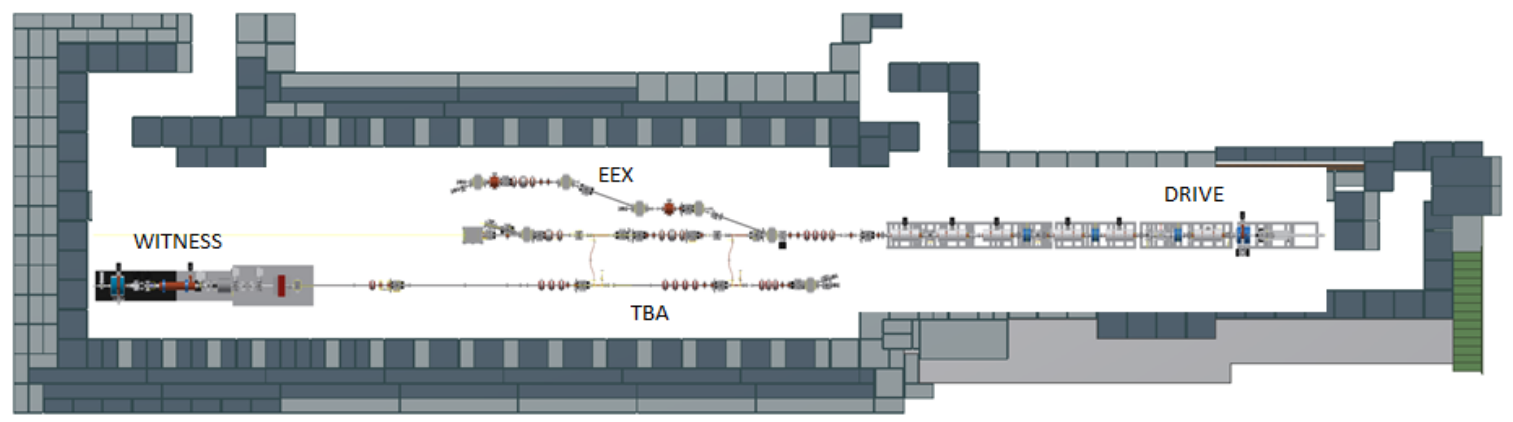
\includegraphics[width=\linewidth]{./images/bunker}
		
	\end{center}
	\caption{AWA Facility bunker and simplified TBA staging layout. 
		The drive beam line (right) supplies high charge bunch trains at \SI{70}{MeV}.
		The witness beam line (left) supplies low charge one bunch at \SI{15}{MeV} }
	\label{fig:bunker}
\end{figure}
\begin{figure}[h]
	\begin{center}
		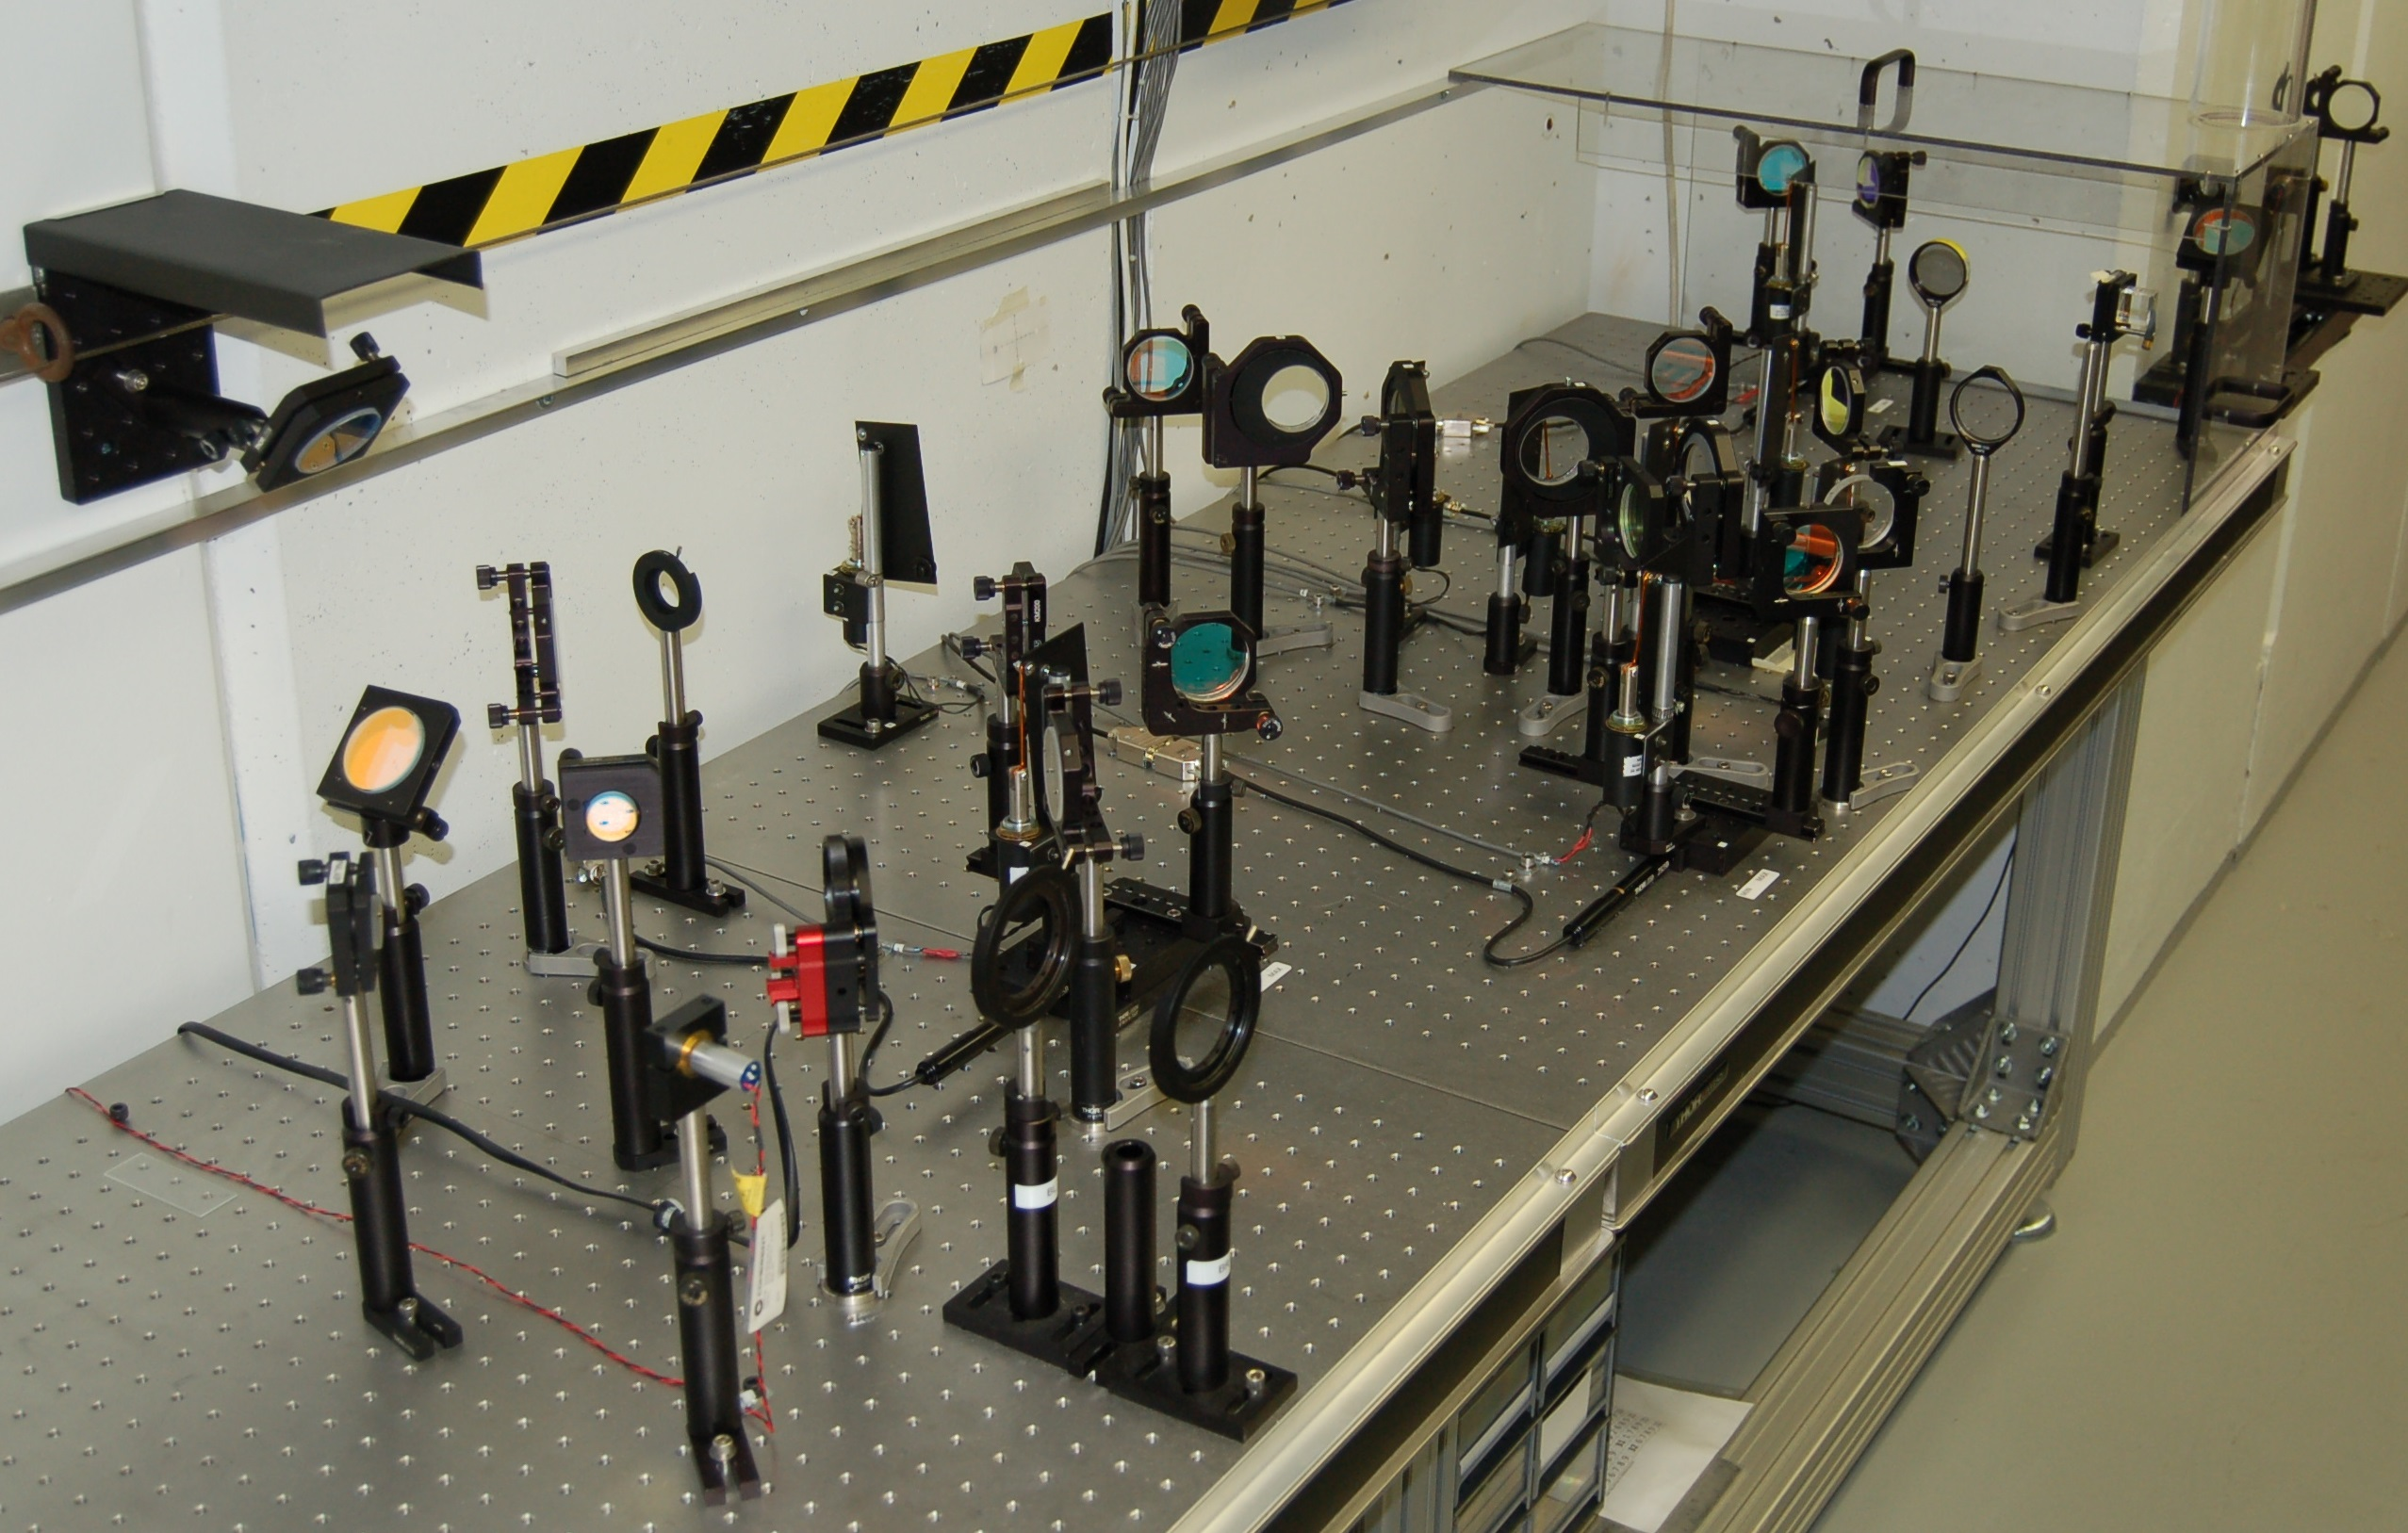
\includegraphics[width=0.5\textwidth]{images/multisplitter}\caption{UV multisplitter optics table.}
	\end{center}
	\label{fig:optics}
\end{figure}
\fi

The witness line rf photoinjector, located on the left side of Figure
1, uses a Mg cathode and the following linac consists of one copper
accelerating cavity. Prior to the multisplitter table, shown in
Fig. \ref{fig:optics}, the laser pulse is split between the drive and witness side.
This set up allows only one bunch per pulse on the witness line. Also
note that the beam from the drive line travels in the opposite direction
than the beam in the witness line. 

%%%%%%%%%%%%%%%%%%%%%%%%%%%%%%%%%%%%%%%%%%%%%%%%%%%%%%%%%%%%%%%%%%%%%%%%%%%%%%%%%%%%%%%%%%%%
%%%%%%%%%%%%%%%%%%%%%%%%%%%%%%%%%%%%%%%%%%%%%%%%%%%%%%%%%%%%%%%%%%%%%%%%%%%%%%%%%%%%%%%%%%%%
\Section{Dielectric Structures}

%%%%%%%%%%%%%%%%%%%%%%%%%%%%%%%%%%%%%%%%%%%%%%%%%%%%%%%%%%%%%%%%%%%%%%%%%%%%%%%%%%%%%%%%%%%%
%%%%%%%%%%%%%%%%%%%%%%%%%%%%%%%%%%%%%%%%%%%%%%%%%%%%%%%%%%%%%%%%%%%%%%%%%%%%%%%%%%%%%%%%%%%%
\Subsection{Power Generation}

\lsnote{Somewhere you need a comprehensive description of simplified staging vesus full staging.  I am not sure it is here, but it should be before you mention simplified staging.}

Currently, all \lsnote{define PETS acronym} PETS and accelerating structures installed in the AWA's
simplified staging scheme are metallic. It has been shown that a few
key equations can demonstrate the relationship between beam parameters
and the resulting \lsnote{\sout{rf} power} generated in the decelerating cavity. This section
borrows heavily from previous work at CLIC and the AWA \cite{key-3,key-8}. 
Starting with the timing, each bunch in the drive train will generate
an rf pulse of finite length in the structure. Each bunch is separated
in time by $T_{b}$, and the \lsnote{average?} beam current can be written as $I=\frac{Q}{T_{b}}$.
\lsnote{define Q, is it the charge per bunch?} The bunches are Gaussian in the longitudinal direction, and the form
factor, $\Phi$, is used to describe\lsnote{\sout{s}} the Gaussian shape by taking
the Fourier transform of the charge distribution: 
\begin{equation}
\Phi=exp\left[\frac{-(k_{z}\sigma_{z})^{2}}{2}\right]
\end{equation}
Where $k_{z}=\frac{2\pi}{\lambda_{z}}$ is the longitudinal wave number
and $\sigma_{z}$ is the rms bunch length. \lsnote{That was confusing.  You said phi was the FT of the charge distribution, but in the equation after that it looks like the charge distribution not the FT}  Note the subscript z \lsnote{indicates \sout{refers to the characteristics of the cavity and bunch in}} the longitudinal
direction. Then using the partial differential equation that relates
the power generated by the wakefield to the change in power over time, \lsnote{I would include the equation}
the power generated by a bunch train can be written as:
\begin{equation} \label{eq:rfpower}
P_{t}(t)=\frac{\omega_{z}\,L^{2}I^{2}}{4\,v_{g}}\frac{R}{Q_{d}}\left(\frac{1-e^{-\alpha L}}{\alpha L}\right)\Phi^{2}
\end{equation}
With $I$ being the beam current as defined above, $\alpha=\frac{\omega}{2Q_{d}v_{g}}$
being the attenuation constant \cite{key-9}, R is the shunt impedance
per unit length, and $Q_{d}$ is the quality factor for the decelerating
structure. \lsnote{You didn't define L or vg} Note, the derivation of equation 4 can be found in reference
\cite{key-8}, and due to the complex geometry of metallic structures,
the value of R/Q is often calculated in electromagnetic codes such
as CST Microwave Studio. 

\lsnote{You probably were intending to do this, but this section should close out with a predicted power generation 
	in the decelerating structures.  The discussion of how that depends on number of bunches in the bunch train should be here as well.}

\Subsection{Accelerating Structures}

\Section{Two Beam Acceleration}

\Section{AWA Design Requirements} \label{sec:requirements}

\lsnote{This is probably where you should have the overview of simple staging versus full staging, and a summary of what was required to go to full staging.  The title of the section should also be changed, maybe `Fully staged two beam acceleration'?}

In order to design and test the desired beam line, three technologies 
new to the AWA were investigated. These include a kicker, septum magnets, 
and non-GA optimization algorithms.

% An example for enumerate
\begin{enumerate}
	\item Kicker Design
	\item Septum Design
	\item Optimization 
\end{enumerate}

% A quotation example
% Every quota must be accompanied by a reference to the source
% in a footnote or in the Bibliography
\begin{quotation}
	test
\end{quotation}






Before final measurements or meaningful simulations can be done, 
a fair amount of set up and preliminary measurements 
must be made and understood. 

%%%%%%%%%%%%%%%%%%%%%%%%%%%%%%%%%%%%%%%%%%%%%%%%%%%%%%%%%%%%%%%%%%%%%%%%%%%%%%%%%%%%%%%%%%%%
%%%%%%%%%%%%%%%%%%%%%%%%%%%%%%%%%%%%%%%%%%%%%%%%%%%%%%%%%%%%%%%%%%%%%%%%%%%%%%%%%%%%%%%%%%%%
\Section{Laser Pulse Train Improvement} \label{sec:uvoptics}
%%%%%%%%%%%%%%%%%%%%%%%%%%%%%%%%%%%%%%%%%%%%%%%%%%%%%%%%%%%%%%%%%%%%%%%%%%%%%%%%%%%%%%%%%%%%
%%%%%%%%%%%%%%%%%%%%%%%%%%%%%%%%%%%%%%%%%%%%%%%%%%%%%%%%%%%%%%%%%%%%%%%%%%%%%%%%%%%%%%%%%%%%

Ideally, to extract maximum power from a series of bunches, each electron bunch should have the same amount of charge.  Improving the laser pulse train intensity distribution improves the electron bunch charge distribution; 
which  helps produce an RF power pulse that is closer to uniform. 
The generated power depends on both the charge and shape of the bunch, as shown in Eq.~\ref{eq:rfpower}. 
Several factors contribute to non-uniformity in the bunches. These include the cathode material
(i.e. slightly different QE along the surface), shot to shot noise in the laser pulse, 
distortion of laser pulses due to traveling through air, and the quality of the optics. 
The last is especially important in determining the intensity of each laser pulse in the train.  
Each splitter has a slightly different value for transmitted (T) and reflected (R) pulses. 

\Subsection{UV Optics} 
In order to generate the drive bunch trains needed for TBA, a UV laser pulse is split 
by five optical splitters into two trains of eight pulses. 
The optics set up is shown in Fig~\ref{fig:optics}. Optical delay lines (two mirrors) near each splitter 
separate pulses in space and time by extending the distance that each pulse travels. 
The length of each delay line is a multiple of the RF frequency, 1.3 GHz. 
In other words, a separation of $1\lambda=\SI{769}{ps}$ between each UV pulse is created. 
This is done to synchronize the laser pulses with the RF supplied to the gun.
In order to achieve equally charged bunches, splitters with a perfect transmission 
to reflection ratio ($T/R = 50/50$) would be required.

\Subsection{UV Splitter Measurements} 
The initially installed splitters were rated at a tolerance of $50\%\pm5\%$.
Measurements of the UV splitters were done to determine the T/R (Transmission to Reflection) ratio for 
each splitter. The measurements took place in the laser room, close to the source of the laser.
The setup included two joule meters; one to measure the raw T/R values and one to measure 
the background. Amplified Spontaneous Emission (ASE), 
is the main contributor to background shot to shot noise in the laser pulse,
and is known to drift with temperature and operating time. 
The ASE value was measured when each T/R measurement was taken, then divided out of the T/R 
measurements to prevent bias due to background drifts. 

Several configurations were tested this way: S-polarization, P-polarization, 
and laser incident on back or front of the coating. 
Whether the laser pulse hit the front or back of the optic
had no measurable effect on the T/R ratio. Polarization did have a significant effect on
the results, which led to more careful observation of this in the future.
The following plot shows the splitters were performing at about 55/45 ratio, 
The results indicated the ratio of reflection to transmission for each splitter ranged from 
$T/R\approx55/45$ to $53/47$. 
This caused an uneven laser intensity distribution, as the bunch intensity depends on the path 
it takes through the multisplitter optics. Pulses that were reflected more than one
time could have significantly lower intensities than other bunches. 
Consider the path of laser pulse four as shown in Fig.~\ref{fig:tikz}. 
The pulse is transmitted through splitters 1, 2, and 4, but is reflected by splitter 3.
\def \delayvertical {1.5}
\def \delayoneleft {7.5}
\def \delaytworight{15}
\def \mycenter{10.0}
\def \labels{6.5}
\def \sone {-0.5}
\def \stwo {\sone+1.5}
\def \sthree {\stwo+1.5}
\def \sfour {\sthree+1.5}
\def \buffer{-4.5}
\iffalse
\begin{figure*}[h]
	\begin{center}		
		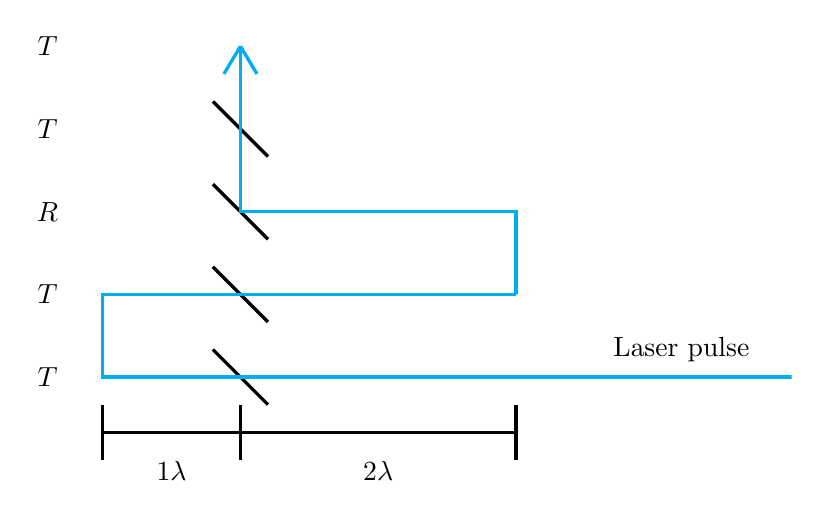
\begin{tikzpicture}[scale=0.7]
		%\node[] at (\labels, 5.5) {Behavior through splitter};
		\node[] at (\labels,6.0) {$T$};
		\node[] at (\labels,4.5) {$T$};
		\node[] at (\labels,3.0) {$R$};
		\node[] at (\labels,1.5) {$T$};
		\node[] at (\labels,0.0) {$T$};
		
		\draw[very thick] (10.5,\sone) -- (9.5,\sone+1); % Splitter 1
		\draw[very thick] (10.5,\stwo) -- (9.5,\stwo+1); % Splitter 2
		\draw[very thick] (10.5,\sthree) -- (9.5,\sthree+1); % Splitter 3
		\draw[very thick] (10.5,\sfour) -- (9.5,\sfour+1); % Splitter 4
		
		\draw[cyan, very thick] (\delayoneleft,0.0) -- (20.0,0.0) % Incoming pulse line
		to(\delayoneleft,0.0) -- (\delayoneleft,\delayvertical) % Delay Leg 1 (a)
		to(\delayoneleft,\delayvertical) -- (15,\delayvertical); % Pulse after delay 1
		
		\draw[cyan,very thick] (\mycenter,\delayvertical*2) -- (\delaytworight,\delayvertical*2)
		to(\delaytworight,\delayvertical) -- (\delaytworight,\delayvertical+1.5)
		to(\mycenter,\delayvertical*2) -- (\mycenter,\delayvertical*4);
		
		\draw[cyan, very thick] (9.7,5.5) -- (10.0,6.0); % arrow head left
		\draw[cyan, very thick] (10.0,6.0) -- (10.3,5.5); % arrow head right
		
		\node[] at (18,0.5) {Laser pulse};
		
		\node[] at (8.75,-1.7) {$1\lambda$};
		\draw[black, very thick] (\delayoneleft, -1) -- (\delaytworight, -1);
		\draw[black, very thick] (\delayoneleft, -1.5) -- (\delayoneleft, -0.5);
		\draw[black, very thick] (\mycenter, -1.5) -- (\mycenter, -0.5);
		
		\node[] at (12.5,-1.7) {$2\lambda$};
		\draw[black, very thick] (\delaytworight, 3.0+\buffer) -- (\delaytworight, 4.0+\buffer);
		
		\end{tikzpicture}
	\end{center} 
	\caption{Example of a laser pulse path through multisplitter. T indicates when the laser pulse is 
		transmitted through the splitter, and R stands for when the laser pulse is reflected by the splitter. 
		The operating wavelength is $\lambda = \SI{23}{cm}$. Bends are accomplished with two UV mirrors, 
		one at each corner of the delay line.}
	\label{fig:tikz}
\end{figure*}
\fi

Each splitter reduces the intensity of the pulse as a new pulse is generated. Expected intensities
can be predicted by using the measured T/R values for each splitter. For example, using $T/R=55/45$,
in Fig~\ref{fig:tikz} the laser pulse is transmitted four times and reflected once: 
\begin{equation}\label{eq:i4}
I_4 =  T \cdot R \cdot T \cdot T \cdot T \cdot I_0 \approx 0.41 I_0
\end{equation}
Therefore, this pulse had a fairly high laser intensity, because it was transmitted multiple times. 
In the worst case, the laser intensity of pulse six: 
\begin{equation}\label{eq:i6}
I_6 =  T \cdot R \cdot R \cdot R \cdot T \cdot  I_0 \approx 0.28 I_0
\end{equation}
These trends were reflected in the electron bunch trains generated in the gun.
As a result, methods to improve the intensity distribution were investigated.

\Subsection{New UV Splitters}
To improve the intensity distribution, splitters with a tolerance of $50\%\pm3\%$ were purchased, 
installed, and the laser energy was measured again. The quality of the splitters was near tolerance 
again, and the bias leaned toward reflection, $T/R \approx 47/53$. With the bias now reversed, 
the trend in intensity distribution was also reversed. The possibility of using a combination 
of splitters from the $\pm3\%$ and $\pm5\%$ sets was explored. 
Using a python script to compare all possible combinations, it was determined that using only 
$\pm3\%$ splitters would result in the lowest variation in intensity. 

\Subsection{Train Intensity Measurements}
To verify the predictions above, and show improvement using the $\pm3\%$,
the intensity of bunches one through eight were measured using four splitters. 
This simplified the experimental set up, and reduced interruption to beam time 
runs which were using the four splitter set up.  
\iffalse
\begin{figure}[h]
	\begin{center}
		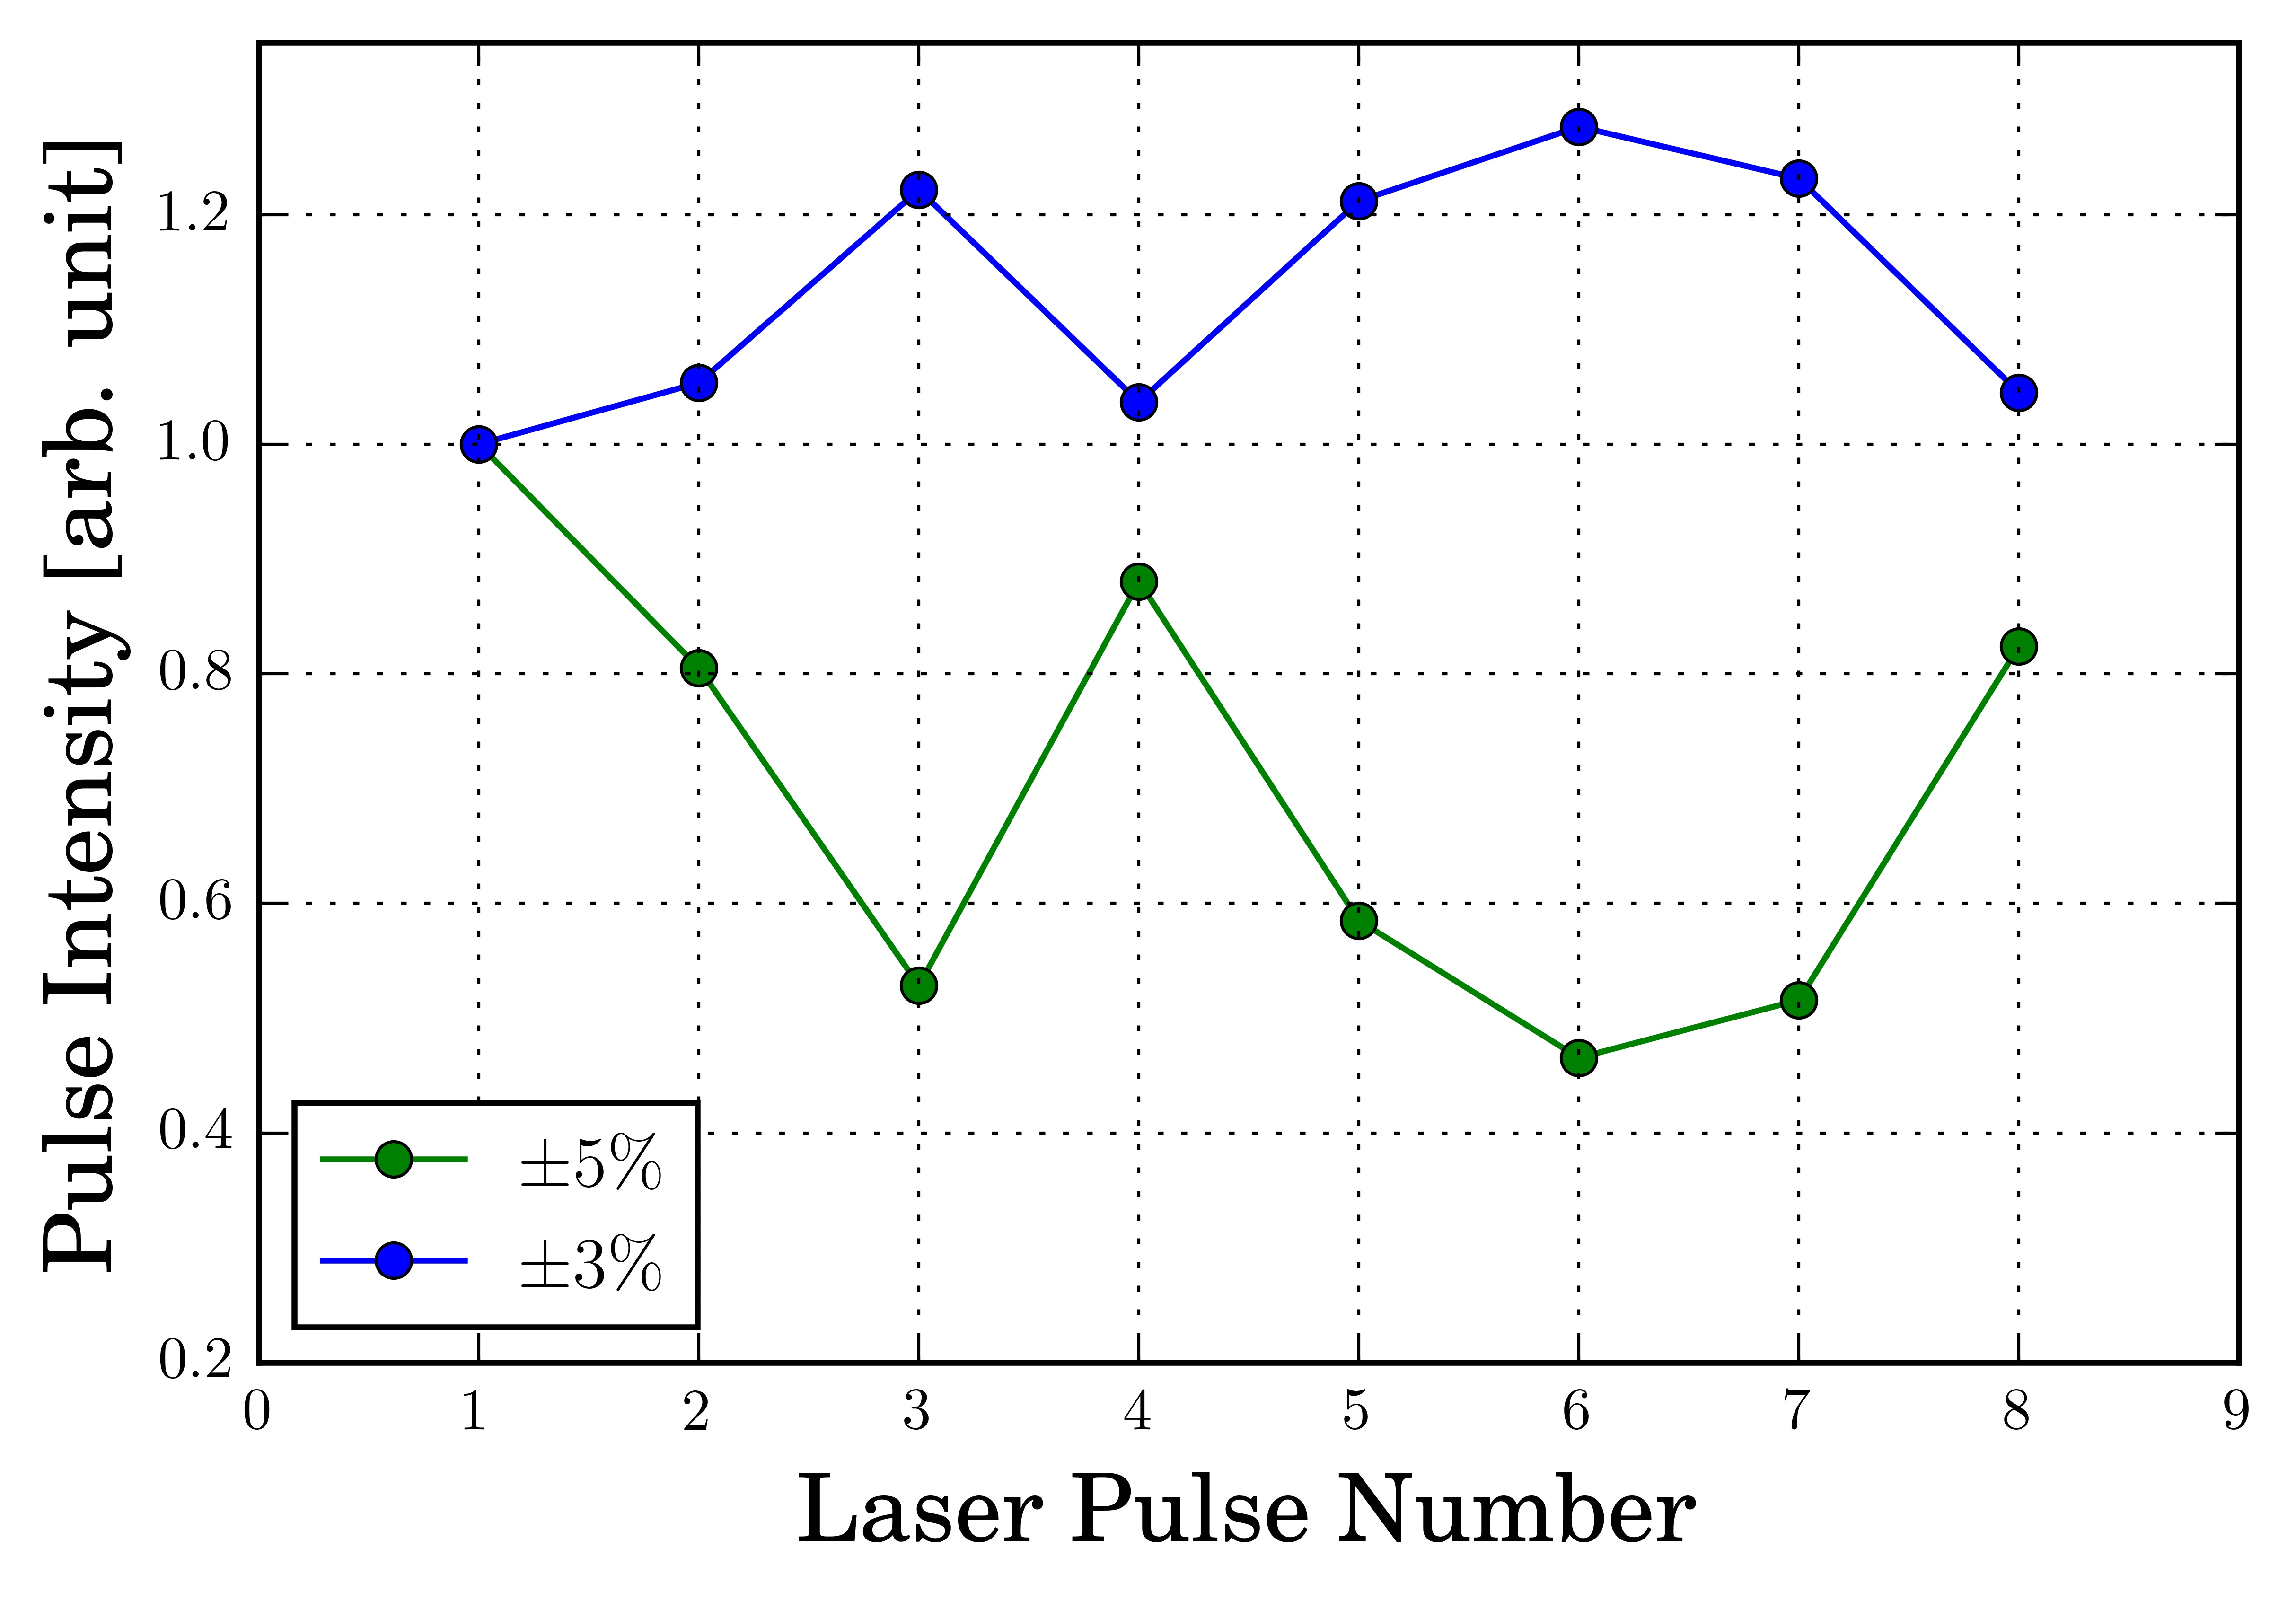
\includegraphics[width=0.8\textwidth]{images/splitter_improvement}\caption{Laser pulse train intensity measurements}
	\end{center}
	\label{fig:origtrain}
\end{figure}
\fi
The predictions in Eqs.~\ref{eq:i4} and~\ref{eq:i6} don't account for mirror losses in the delay legs, 
so we expect a lower value in experiment. To do a quick check on whether or not these results are 
expected, consider laser pulse one and only four splitters (as was the experimental set up). 
Laser pulse one has a similar path to laser pulse four (Eq.~\ref{eq:i4}). 

\begin{equation}
I_1 = R \cdot T \cdot T \cdot T \cdot I_0 
\end{equation}

Given about $\pm10\%$ mirror loss in the delay legs, we expect laser pulse one and four 
to be roughly the same intensity. This is shown in Fig.~\ref{fig:origtrain}. With the same 
logic, we expect pulse six to have the largest deviation from pulse one, as it is reflected 
three times and transmitted once in the four splitter set up. This expectation is also 
confirmed by the results in Fig.~\ref{fig:origtrain}.  \lsnote{You achieved a significant improvement in the uniformity of the laser pulse train, as can be seen in the figure.  Even though it can be seen in the figure, you should wrap up the section with a quantitative statement about the improvement you achieved, along with a summary sentence on how you achieved it.  Something like, `Through the use of optics with tighter specifications, and sorting of the optical elements, an improvement in laser pulse uniformity of bla percent was achieved.'}  

%%%%%%%%%%%%%%%%%%%%%%%%%%%%%%%%%%%%%%%%%%%%%%%%%%%%%%%%%%%%%%%%%%%%%%%%%%%%%%%%%%%%%%%%%%%%
%%%%%%%%%%%%%%%%%%%%%%%%%%%%%%%%%%%%%%%%%%%%%%%%%%%%%%%%%%%%%%%%%%%%%%%%%%%%%%%%%%%%%%%%%%%%
\Section{RF Measurements}
%%%%%%%%%%%%%%%%%%%%%%%%%%%%%%%%%%%%%%%%%%%%%%%%%%%%%%%%%%%%%%%%%%%%%%%%%%%%%%%%%%%%%%%%%%%%
%%%%%%%%%%%%%%%%%%%%%%%%%%%%%%%%%%%%%%%%%%%%%%%%%%%%%%%%%%%%%%%%%%%%%%%%%%%%%%%%%%%%%%%%%%%%
In order to accurately simulate the RF fields in the cavities on the drive and witness line, 
a set of detailed measurements were done to determine the power in each RF cavity.
This includes power and energy measurements of the drive gun, and linac tanks 
one through 6 on the drive line.
\lsnote{You have a gun section below, so you should mention that in this paragraph as well as the cavities.}

\Subsection{Cable Calibration} \label{cablecal}
There is a significant length of cable that connects the cavities to the control room.
To calibrate these cables, a signal generator was placed in the tunnel. 
Then a signal was propagated to the control room where it was 
measured and compared to the original power measurement in the tunnel. 
\begin{figure*}[h]
	\begin{center}	
		\begin{circuitikz}[scale=0.7]
            \draw (0,0) to[csV=] (2,0);
            \node[align=center] at (0.8,2.0) {Signal \\ Generator};
            
			%Control room or power meter
			\def \leftside {3}
			\def \topbox {0.75}
			\def \botbox {-0.75}
			\draw (2.0, 0) -- (\leftside, 0);
			\draw[fill=white, ultra thick, rounded corners =0.1cm] (\leftside,\botbox)rectangle  
			({\leftside+3},\topbox) node[pos=0.5, align=center] {Meter};           
		\end{circuitikz}
    \end{center} 
\caption{Refrence power reading was taken while power meter was directly connected to the 
signal generator. The resulting power was $P_s=\SI{-8.92}{dBm}$}
\label{fig:signalgenerator}
\end{figure*}


\def \delayvertical {1.5}
\iftrue
\begin{figure*}[h]
	\begin{center}	
		\begin{circuitikz}[scale=0.7]
			
			\draw (0,0) to[csV=] (2,0);
			\node[align=center] at (0.8,2.0) {Signal \\ Generator};
			%Short blue RF cable 
			\node[] at (3.5,1) {$C_{1}$};
			\node[tlinestub] at (2,0){};
			\node[] at (3.5,-1) {};
			
			%Long RF cable
			\node[] at (7,1) {$C_{2}$};
			\node[tlinestub] at (5.5,0){};
			
			%Short yellow RF cable
			\node[] at (9.5,1) {$C_{3}$};
			\node[tlinestub] at (8.1,0){};
			%\draw[] (4.6,0) to[short,-] ++(1,0);
			\draw (4.6, 0) -- (5.6, 0);
			%10 dB attenuator
			\draw (10.7,0) to[R=$\SI{10}{dB}$, color=red] (14,0);
			
			%Control room or power meter
			\def \leftside {14}
			\def \topbox {0.75}
			\def \botbox {-0.75}
			%\draw (10.75, 0) -- (\leftside, 0);
			\draw[fill=white, ultra thick, rounded corners =0.1cm] (\leftside,\botbox)rectangle  
			({\leftside+3},\topbox) node[pos=0.5, align=center] {Meter};
		\end{circuitikz}
	\end{center} 
	\caption{Experimental set up when calibrating the cables from gun to control room. 
		Where $C_1$ is a short blue heliax, $C_2$ is a long heliax to the control room, 
		and $C_3$ is a short yellow heliax to the 6 GHz scope or power meter.}
	\label{fig:tikzcalibration}
\end{figure*}
\fi
The power reading in the control room was $P_c = \SI{-9.48}{dBm}$, and the power reading in 
the tunnel from the signal generator was $P_s = \SI{-8.92}{dBm}$, so the
attenuation is $\SI{0.56}{dB}$. However, one more cable needs to be accounted for and 
subtracted from the overall attenuation. A short blue heliax was used to connect the 
signal generator to the control room cables, as shown in Fig.~\ref{fig:tikzcalibration}.
This cable not normally connected to the control room as shown in Fig.~\ref{fig:tikzdrivegun}. \lsnote{You should finish the thought - how much attenuation from the Heliax, and what is the adjusted correction?}


\Subsection{Drive Gun Measurements}\label{gunenergy}
After the cable calibration, the set up was returned to typical rf conditions as 
shown in Fig.~\ref{fig:tikzdrivegun}. This includes $\SI{53.2}{dB}$ from the pick 
up probe itself, a $\SI{36}{dB}$ additional attenuation connected to the 
drive gun pick up probe, followed by a long heliax to the 
control room. The signal split in the control room with a mini-circuit ZFRSC-123-S+. 
One port is used for Low Level RF (LLRF) control, and the other port was connected to a short 
heliax, $C_3$, then to a $\SI{10}{dB}$ attenuator and finally to the 
power meter. Normally a load is placed at port two when no power meter is connected. 
Next, the klystrons and phase shifters were set to supply 
max power to the gun, typical of TBA running conditions. 
\def \delayvertical {1.5}
\iftrue
\begin{figure*}[h]
	\begin{center}		
		\begin{circuitikz}[scale=0.7]
			\def \leftside {17.0}
			\def \topbox {0.75}
			\def \botbox {-0.75}
			
			\node[] at (0.8,1.3) {Gun};
			\draw (0,0) to[csV=] (2,0);
			
			\def \gunright {2}
			%Attenuators
			%\node at (2, -0.50) {$P_1$};
			%\node at (5, -0.50) {$P_2$};
			
			\draw (\gunright,0) to[R=$\SI{53.2}{dB}$, color=red] (\gunright+2,0);
			\draw (\gunright+2.5,0) to[R=$\SI{36}{dB}$, color=red] (\gunright+4.5,0);
			\draw[] (\gunright+2.0,0) to[short,-] ++(0.5,0);
			%Long RF cable
			
			\node[] at (\gunright+6,1) {$C_{2}$};
			\node[tlinestub] at (\gunright+4.5,0){};
			\draw (9.0, 0) -- (10.0, 0);
			\draw[fill=white, ultra thick, rounded corners =0.1cm] (\gunright+8.0,\botbox)rectangle  
			%splitter
			({\gunright+11.0},\topbox) node[pos=0.5, align=center] {Splitter};
			\draw (11.5, 0.7) -- (11.5, 2);
			\node[] at (11.5, 2.5) {LLRF};
			
			%Short yellow RF cable
			\draw (13.0, 0) -- (13.5, 0);
			\node[] at (\gunright+13.0,1) {$C_{3}$};
			\node[tlinestub] at (\gunright+11.5,0){};
						
			%10 dB attenuator
			\draw (16.0, 0) -- (16.5, 0);
			\draw (\gunright+14.5,0) to[R=$\SI{10}{dB}$, color=red] (\gunright+16.5,0);
			
			%Control room or power meter
			\draw (18.5, 0) -- (\leftside+2, 0);
			\draw[fill=white, ultra thick, rounded corners =0.1cm] (\leftside+2,\botbox)rectangle  
			({\leftside+5},\topbox) node[pos=0.5, align=center] {Meter};
		\end{circuitikz}
	\end{center} 
	\caption{Experimental set up when measuring power from gun to control room. 
		Where $\SI{53.2}{dB}$ of attenuation is due to the gun probe itself, 
		$\SI{36}{dB}$ of additional attenuation is attached to gun pick up probe cable in the tunnel, 
		$C_2$ is a long heliax to the control room. The $\SI{9.5}{dB}$  splitter sends half the signal to the   
		low level RF (LLRF) control system, and half to the power meter. 
		$C_3$ is a short yellow heliax that connects the meter to the splitter and on to the 6 GHz scope or power meter.}
	\label{fig:tikzdrivegun}
\end{figure*}
\fi

Using the set up in Fig.~\ref{fig:tikzdrivegun}, the power meter measured  $P_{g} = \SI{-14.18}{dBm}$
in the control room. Now we must account for attenuation to know the true power
signal out of the gun. 
\begin{equation}
P_1 = P_r + A_1 + C_2 + S + C_3 + A_2 + P_g
\end{equation}
\begin{equation}
P_g \, \SI{}{[dBm]} = \SI{53.2}{dB} + \SI{36}{dB} + \SI{0.56}{dB} + \SI{9.5}{dB}+ \SI{0.56}{dB} + \SI{10}{dB} + \SI{14.18}{dBm} = \SI{124}{dBm} or 95.6?
\end{equation}

Then converting to a more convenient unit: 
\begin{equation}
P \, \SI{}{[dBm]} = 10 \cdot \log{\frac{P \, \SI{}{[mW]}}{\SI{1}{[mW]}}}
\end{equation}
\begin{equation} \label{eq:dbmtomw}
P \, \SI{}{[mW]} = \SI{1}{[mW]} \cdot 10^{\frac{P \, [\SI{}{dBm}]}{\SI{10}{}}}
\end{equation}
\begin{equation} 
P_2 = 10^{\SI{9.56}{dBm}} \cdot  \SI{1}{[mW]} = 3.6 \, \SI{}{[MW]} 
\end{equation}

\Subsection{Linac Cavity Measurements}
There are six linear accelerating (linac) cavities after the gun. 
Each are connected to the control room in the same way as the gun. 
The only differences are in the attenuation at the pick up probe and 
the splitter attenuation. Using the methods in section \ref{gunenergy}, 
and the attenuation values, we can calculate the power in each linac cavity:

\begin{table} %or [hbt] ?
	\caption{\label{tab:powerlinac} Power and attenuation values for the 
		linac cavities. Note that all cavities have an additional 
		\SI{33}{dB} attenuation added after the probe.}
	\begin{center}
		\begin{tabular}{ccccc}
			\toprule
			\textbf{Cavity} & \textbf{Probe Att.} & \textbf{Splitter Att.} & \textbf{Power Meter 1}  & \textbf{Power Meter 2} \\
			\midrule
			Gun & \SI{-53.2}{dB}& $9.5 \pm \SI{0.3}{dBm}$ & \SI{-14.18}{dBm} & \SI{-3.86}{dBm}  \\
			2 & \SI{}{dB}       & $9.5 \pm \SI{0.3}{dBm}$ & \SI{-18.88}{dBm} & \SI{-9.6}{dBm}  \\
			3 & \SI{}{dB}       & $4.0 \pm \SI{1.0}{dBm}$ & \SI{-12.24}{dBm} & \SI{-1.54}{dBm}  \\
			4 & \SI{-61.95}{dB} & $9.5 \pm \SI{0.3}{dBm}$ & \SI{-18.89}{dBm} & \SI{-10.11}{dBm}  \\
			5 & \SI{}{dB}       & $9.5 \pm \SI{0.3}{dBm}$ & \SI{-17.76}{dBm} & \SI{-8.39}{dBm}  \\
			6 & \SI{-61}{dB}    & \SI{}{dB} 			  & \SI{-14.32}{dBm} & \SI{-2.83}{dBm} \\
			\bottomrule
		\end{tabular}
	\end{center}
\end{table}

\nrnote{Move this to appendix later:}
	
	Power readings long yellow cable:
$G$ readings:$[-14.18]$	

$L_2$ readings:$[-18.88]$

$L_3$ readings:$[-12.21,-12.38, -12.24, -12.24, -12.24, -12.39, -12.24, -12.24]$

$L_4$ readings:$[-18.84]$

$L_5$ readings:$[-17.76]$

$L_6$ readings:$[-14.36,-14.28,-14.25,-14.30,-14.35,-14.33]$

Power readings short yellow cable:
$G$ readings:$[-3.88, -3.83]$	

$L_2$ readings:$[-9.6]$

$L_3$ readings:$[-1.54]$

$L_4$ readings:$[-10.15, -10.13, -10.10, -10.07]$

$L_5$ readings:$[-8.46,-8.31]$

$L_6$ readings:$[-2.84, -2.84, -2.81, -2.82]$

Site for new splitters: %\url{https://www.minicircuits.com/pdfs/ZFRSC-123+.pdf}
Site for old splitters: %\url{https://www.minicircuits.com/pdfs/ZAPD-2-252+.pdf}

\nrnote{end of appendix info}

\begin{equation}
P_1 = \SI{-61.95}{dBm} + \SI{33}{dB} + \SI{0.56}{dB} + \SI{9.5}{dBm} +\SI{10}{dBm}
\end{equation}



%%%%%%%%%%%%%%%%%%%%%%%%%%%%%%%%%%%%%%%%%%%%%%%%%%%%%%%%%%%%%%%%%%%%%%%%%%%%%%%%%%%%%%%%%%%%
%%%%%%%%%%%%%%%%%%%%%%%%%%%%%%%%%%%%%%%%%%%%%%%%%%%%%%%%%%%%%%%%%%%%%%%%%%%%%%%%%%%%%%%%%%%%
\Section{Energy Measurements} \label{sec:dipolecal}
%%%%%%%%%%%%%%%%%%%%%%%%%%%%%%%%%%%%%%%%%%%%%%%%%%%%%%%%%%%%%%%%%%%%%%%%%%%%%%%%%%%%%%%%%%%%
%%%%%%%%%%%%%%%%%%%%%%%%%%%%%%%%%%%%%%%%%%%%%%%%%%%%%%%%%%%%%%%%%%%%%%%%%%%%%%%%%%%%%%%%%%%%
Energy measurements at the AWA are done with a traditional 
spectrometer. This includes a dipole magnet and two Yittrium 
Aluminum Garnet (YAG) screens as shown in Fig~\ref{fig:spectrometer}.

\begin{figure*}[h]
	\begin{center}		
		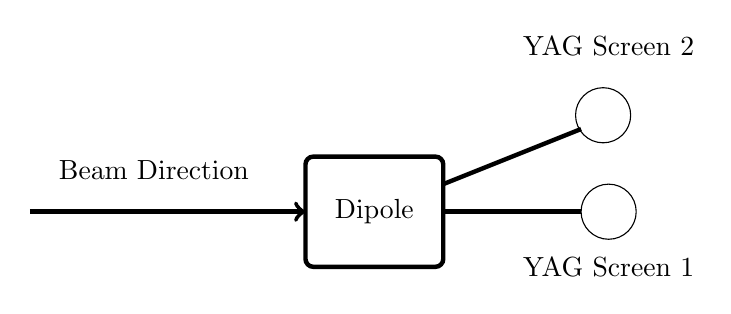
\begin{tikzpicture}[scale=0.7]
			
			\node[] at (2.25,0.75) {Beam Direction};
			\draw[ultra thick, ->] (0,0) -- (5.0, 0.0);
			
			\draw[fill=white, ultra thick, rounded corners =0.1cm] (5.0,1.0)rectangle  
			(7.5,-1.0) node[pos=0.5, align=center] {Dipole};
			
			\draw[ultra thick] (7.5, 0.0) -- (10.0, 0.0);
			\draw[ultra thick] (7.5, 0.5) -- (10.0, 1.5);
						
			\node[] at (10.5, 3) {YAG Screen 2};
			\draw (10.4,1.75) circle (0.5cm);
			
			\node[] at (10.5, -1.0) {YAG Screen 1};
			\draw (10.5,0) circle (0.5cm);
			
		\end{tikzpicture}
	\end{center} 
	\caption{Spectrometer set up in all cases at AWA.}
	\label{fig:spectrometer}
\end{figure*}

\Subsection{Energy Measurement Procedure}
Taking an energy measurement requires a beam trajectory
that is centered through the dipole. Otherwise, the beam 
may experience excessive non-uniform fields 
if it enters the dipole off-axis. The centering is done with two 
quads before the dipole. The center is found by focusing 
in the x-direction, and then the y-direction. If the beam 
moves to the left or the right as it is being focused, 
the quad is "steering", and the beam is entering the magnets off-axis.
Once the beam is centered through the quads on YAG screen 1, 
the dipole is then turned on to bend the beam.
The two YAG screens are positioned so that when the dipole is off, 
a centered beam will hit YAG screen 1. When the dipole is turned
on, the beam will appear at the center of YAG screen 2 when the 
beam is bent $20^\circ$. In this way, the dipole strength can 
then be used to determine the beam energy.

\Subsection{Energy Calculation}
Based on the procedure above, there is one number which we 
use to back calculate the mean energy. The amount of current
supplied to the dipole is represented by the number of "counts"
keyed into the control system. A counts to current line
is calculated given the measurements shown in Table \ref{tab:counts}
\begin{table}
\begin{center}
	\begin{tabular}{||c c||} 
		\hline
		Counts & Current [A] \\ [0.5ex] 
		\hline\hline
		1000 & 3.7 \\ 
		\hline
		5000 & 18.8 \\
		\hline
		10000 & 37.5 \\
		\hline
		15000 & 56.3 \\
		\hline
		
	\end{tabular}
\end{center}
\caption{Counts to current data for the first dipole in the drive beam line.}
\end{table}\label{tab:counts}
Then the B-field is calculated given the current: 
\begin{equation}
	\SI{}{B\,[T]} = (180.9708\cdot \SI{}{I\,[A]} - 7.2053)\cdot 10^{-4}
\end{equation}
There are a few geometric calculations that need to be done using the magnetic field value. 
before we can calculate the energy. 
The radius of curvature, $\rho$, 
can be calculated using the effective length of the dipole, L, and bending angle, $\theta$.
\begin{equation}
	\rho = \frac{L}{2\cdot \sin(\frac{\theta}{2})}
\end{equation}
Using $\rho$, and geometry, we can also estimate the x offset of the
beam after the dipole: 
\begin{equation}
	\Delta x = \rho \left( 1- \cos\theta \right)
\end{equation}
Using this and the famous relationship, $B\rho$ \cite{Wiedemann},
we can relate the B field and the beam momentum. 
\begin{equation}
	\SI{}{p\,\left[\frac{MeV}{c}\right]} = \frac{B\cdot \rho}{3.3356}\cdot 10^3
\end{equation}
We can then calculate the total energy by including the rest mass of the electrons \cite{Griffiths}:
\begin{equation}
	\SI{}{E\,[MeV]} = \sqrt{0.511^2+p^2}
\end{equation}\label{eq:energy}

\Subsubsection{Hard Edge Dipole Example}
\nrnote{this example is more of a double check and reference for me than for the reader...}
Since this calculation is used several time throughout the 
beam line for different magnets, lets consider a hard edge 
dipole, to show how the above equations can be used to determine
the x offset after the magnet, and the beam energy. 

Let's define the dipole length, $L=\SI{0.2}{[m]}$, angle, $\theta=\SI{20}{degrees}$. 
The corresponding radius is $\rho = \SI{0.5759}{[m]}$. With these values we can now 
calculate the offset, $\Delta x \approx \SI{34}{[mm]}$, which is confirmed by OPAL. 

\nrnote{not sure if I want to include energy since it depends on measured counts....}
Given a count of  energy of $\SI{64.8}{[MeV]}$ given measured counts of 

%%%%%%%%%%%%%%%%%%%%%%%%%%%%%%%%%%%%%%%%%%%%%%%%%%%%%%%%%%%%%%%%%%%%%%%%%%%%%%%%
%%%%%%%%%%%%%%%%%%%%%%%%%%%%%%%%%%%%%%%%%%%%%%%%%%%%%%%%%%%%%%%%%%%%%%%%%%%%%%%%
\Section{Transverse Beam Size Measurements} \label{sec:beamsize}
%%%%%%%%%%%%%%%%%%%%%%%%%%%%%%%%%%%%%%%%%%%%%%%%%%%%%%%%%%%%%%%%%%%%%%%%%%%%%%%%
%%%%%%%%%%%%%%%%%%%%%%%%%%%%%%%%%%%%%%%%%%%%%%%%%%%%%%%%%%%%%%%%%%%%%%%%%%%%%%%%
Beam size measurements are taken by using YAG screens at multiple z locations along the beam line.
The code used to produce all the following images can be found at this git repository:

\url{https://github.com/nneveu/imageProcessing}

\Subsection{Capturing Images}
\nrnote{Add tikz picture here to show how camera is pointed into beam line with mirrors}

\Subsection{Post Processing Images}
A python script was written to take beam images and convert them to profiles in the x and y direction.
This is done in a series of steps, and requires that one or more images can be used as a 
background image and fiducial image. A background image must capture any dark current 
that is present when the beam is not hitting the YAG screen. The fiducial image must 
clearly show the edges of the YAG screen so that a mm/pixel conversion can be calculated.
The following steps detail the post processing from raw image to transverse beam size estimate.

\Subsubsection{Step 1: Calculating the fiducial}

\Subsubsection{Step 2: Remove background intensity}

\Subsubsection{Step 3: Calculate x and y beam profile}

\Subsubsection{Step 4: Fit profile to calculate beam size}


\Section{Bunch Length Measurements}

\Subsection{Measurement Technique}
In order to measure the bunch length, we performed an autocorrelation scan
of the CTR produced by the electron distribution \cite{Happek, WBarry}.
In brief, the CTR is transported into a Michelson interferometer (MI)
where it's split and directed into two MI arms with a half-transparent pellicle \cite{PhysRevSTAB.9.082801}. 
The CTR beams are then combined together at the exit of the MI with the variable path difference.
The resulting CTR intensity is registered with a liquid helium cooled IR Labs
bolometer \cite{IRlabs} as a function of path difference.
The path difference is then converted into time as $\Delta \tau = 2 \Delta x$.
The resulting FWHM bunch duration is determined from the Gaussian fit of 
the interferogram; see Fig. \ref{interferogram}.
\begin{figure}
	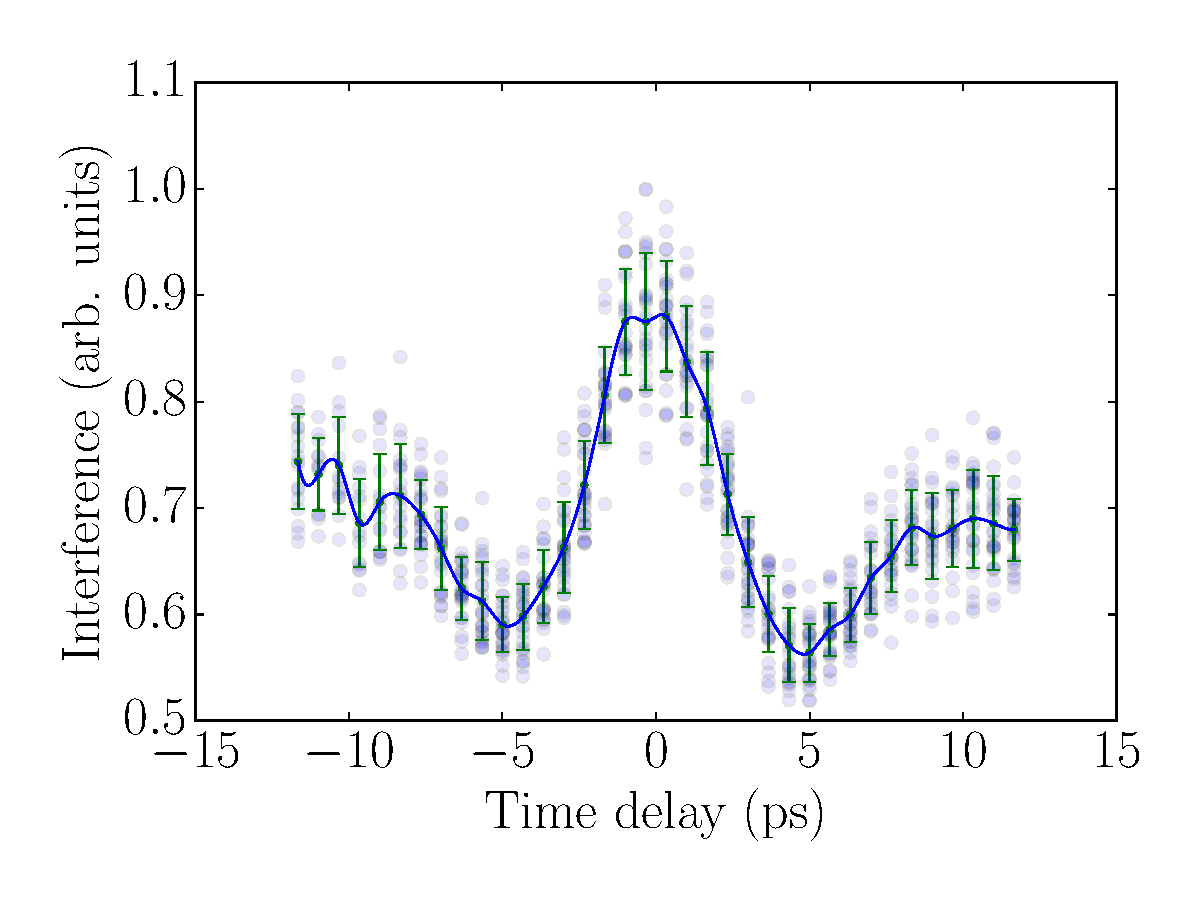
\includegraphics[width=1.0\linewidth]{images/THPMF048f1}
	\caption{An example interferogram for Q=30 nC and laser pulse FWHM of 1.5 ps.}
	\label{interferogram}
\end{figure}
To alleviate the effect of charge fluctuations, we recorded 15 bolometer values for each data point.
The values were then averaged and the errorbars were deduced from the data. The data points
outside of the 3$\sigma$ bracket were considered as outliers and discarded. The resulting
interference pattern as a function of time delay in the MI is similar to that presented in Fig.~\ref{interferogram}.

\begin{figure*}[hbt]
	\centering
	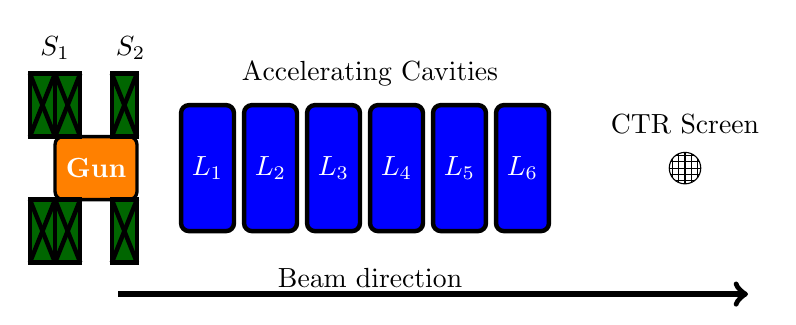
\begin{tikzpicture}[scale=0.8, text=black]
	\def \gunleft {-1.0}
\def \gunright {0.3}
\def \loneright {1.0}
\def \ltworight {2.0}
\def \lthreeright {3.0}
\def \lfourright {4.0}
\def \lfiveright {5.0}
\def \lsixright {6.0}
\def \quadone {7.5}

%Line between kicker and septum
\node[] at (4.0,-0.75) {Beam direction};
\draw[line width=0.75mm, ->] (0.0,-1.0) -- (10,-1.0);

\draw[fill=orange, very thick, rounded corners =0.1cm] (\gunleft,0.5)rectangle (\gunright,1.5) node[pos=.5, white] {\textbf{Gun}} ;
%S1
\node[] at (-1,2.9) {$S_1$};
\draw[ultra thick, fill=black!60!green] (-1.4,-0.5)rectangle  (-1.0,0.5) node[pos=.5, white] {} ;
\draw[black, ultra thick] (-1.4,-0.5) -- (-1.0,0.5);
\draw[black, ultra thick] (-1.4,0.5) -- (-1.0,-0.5);
\draw[ultra thick, fill=black!60!green] (-1.4,1.5)rectangle  (-1.0,2.5) node[pos=.5, white] {} ;
\draw[black, ultra thick] (-1.4,1.5) -- (-1.0,2.5);
\draw[black, ultra thick] (-1.4,2.5) -- (-1.0,1.5);
%S2
\draw[ultra thick, fill=black!60!green] (-1.0,-0.5)rectangle  (-0.6,0.5) node[pos=.5, white] {} ;
\draw[black, ultra thick] (-1.0,-0.5) -- (-0.6,0.5);
\draw[black, ultra thick] (-1.0,0.5) -- (-0.6,-0.5);
\draw[ultra thick, fill=black!60!green] (-1.0,1.5)rectangle  (-0.6,2.5) node[pos=.5, white] {} ;
\draw[black, ultra thick] (-1.0,1.5) -- (-0.6,2.5);
\draw[black, ultra thick] (-1.0,2.5) -- (-0.6,1.5);

%S3
\node[] at (0.2,2.9) {$S_2$};
\draw[ultra thick, fill=black!60!green] (-0.1,-0.5) rectangle  (0.3,0.5) node[pos=.5, white] {};
\draw[black, ultra thick] (-0.1,-0.5) -- (0.3,0.5);
\draw[black, ultra thick] (-0.1,0.5) -- (0.3,-0.5);
\draw[ultra thick, fill=black!60!green] (-0.1,1.5) rectangle  (0.3,2.5) node[pos=.5, white] {};
\draw[black, ultra thick] (-0.1,1.5) -- (0.3,2.5);
\draw[black, ultra thick] (-0.1,2.5) -- (0.3,1.5);
%Linac drawings 
\node[] at (4,2.5) {Accelerating Cavities};
\draw[fill=blue, ultra thick, rounded corners =0.1cm] (\loneright,0)rectangle  ({\loneright+0.84},2) node[pos=.5, white] {$L_1$} ;
\draw[fill=blue, ultra thick, rounded corners =0.1cm] (\ltworight,0)rectangle  ({\ltworight+0.84},2) node[pos=.5, white] {$L_2$};
\draw[fill=blue, ultra thick, rounded corners =0.1cm] (\lthreeright,0)rectangle ({\lthreeright+0.84},2) node[pos=.5, white] {$L_3$};
\draw[fill=blue, ultra thick, rounded corners =0.1cm] (\lfourright,0)rectangle ({\lfourright+0.84},2) node[pos=.5, white] {$L_4$};
\draw[fill=blue, ultra thick, rounded corners =0.1cm] (\lfiveright,0)rectangle ({\lfiveright+0.84},2) node[pos=.5, white] {$L_5$};
\draw[fill=blue, ultra thick, rounded corners =0.1cm] (\lsixright,0)rectangle ({\lsixright+0.84},2) node[pos=.5, white] {$L_6$};

%current optimization point
%\node[draw, fill=yellow, star, star points=5, star point ratio=0.6, minimum size=0.1cm]
%at (12.5,1.0) {$z_1$};
\node[] at (9,1.7) {CTR Screen};
\clip[draw] (9,1) circle (0.25cm);
\draw[step=1mm] (-1,-1) grid (10,10);

%Line between kicker and septum
\draw[very thick] (13.25,0.2) -- (14.5,-0.5);


%Line between septum and dipole
\draw[very thick] (15.6,-0.5) -- (16.5,-0.5);




	\end{tikzpicture}	
	\caption{Beam line layout at the AWA.}
	\label{beamline}
\end{figure*}
\Subsection{Experimental Setup}
The beam line layout is shown in Fig.~\ref{beamline}. 
Bunches were allowed to propagate freely to the 
CTR screen. The only focusing elements used were solenoids $S_1$ and
$S_2$. As the bunches passed the CTR screen, light was
emitted through a window located next to the screen, 
as shown in Fig.~\ref{bolo}. A slit was used to prevent
background x-rays from reaching the bolometer.
After passing the slit, the CTR propagated to the 
interferometer also shown in Fig.~\ref{bolo}. 
A remotely movable stage inside the interferometer was swept, 
and the resulting combined signal fed to the bolometer. 
%The bolometer was cooled with liquid helium. 
Periodic refilling of the helium was required throughout the day in order
to keep the bolometer at \SI{4}{K}. The bolometer sensitivity knob was at position ``1'' and
the gain set to 200.
For the case of 1 nC electrons beams, the laser transverse profile was homogenized prior to the vacuum injection \cite{PhysRevAccelBeams.20.103404}.
To produce high-charge 30 nC beams, we implemented an additional laser beamline that bypasses the homogenizer due to the losses in the 
MLA and relay optics.

\begin{figure}
	\begin{tikzpicture}[every node/.style={anchor=south west,inner sep=0pt},x=1mm, y=1mm,]   
	\node (fig1) at (0,0)
	{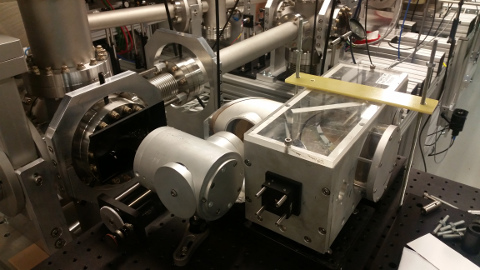
\includegraphics[width=0.5\textwidth]{images/THPMF048f3}};
	\node[fill=white, inner sep=2pt] (txt2) at (35,15) {Interferometer};
	\node[fill=white, inner sep=2pt, rotate=26] (txt2) at (18,19.5) {Slit};	
	\node[fill=white, inner sep=2pt, rotate=20] (txt2) at (13,27) {Window};
	
	\node (fig2) at (0,-50)
	{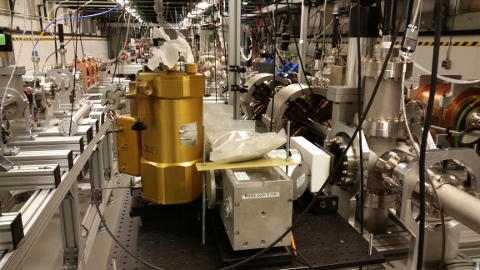
\includegraphics[width=0.5\textwidth]{images/THPMF048f4}};
	\node[fill=white, inner sep=2pt] (txt2) at (35,-42) {Interferometer};	
	\node[fill=white, inner sep=2pt] (txt2) at (55,-25) {Window};	
	\node[fill=white, inner sep=2pt] (txt2) at (22,-15) {Bolometer};
	\end{tikzpicture}
	\caption{IR labs bolometer and MI interferometer used in the experiment
		to capture CTR light as it exited a window on the beam line. }
	%\label{inter}
	%\caption{Bolometer. }
	\label{bolo}
\end{figure}


\Subsection{Simulations}
Simulations of the AWA beam line shown in Fig.~\ref{beamline}
were performed with the code and OPAL~\cite{opal}.
The gun, accelerating cavities, and solenoids were modeled with 2D
Poisson/Superfish~\cite{fish} files. All field maps were in the T7 format.
Input parameters for the simulations are shown in Table~\ref{simparam}.
Note that on crest refers to the phase of max energy gain.
In the case of the gun, a -~$5^{\circ}$ phase is measured 
w.r.t the peak rf voltage.
\begin{table}[hbt]
	%   \vspace*{-.5\baselineskip}
	\centering
	\caption{Simulation Parameters}
	\begin{tabular}{lcc}
		\toprule
		\textbf{Parameter} & \textbf{Low Charge}  & \textbf{High Charge} \\
		\midrule
		Charge       & 0.3, 0.7, \SI{1.3}{nC}        & \SI{30}{nC}    \\ %[3pt]
		Gun Gradient & \SI{65}{MV/m}     & \SI{65}{MV/m}  \\ %[3pt]
		Gun Phase    & \SI{0}{}$^{\circ}$ & \SI{-5}{}$^{\circ}$ \\		 
		$S_1$        & \SI{230}{A}		 & \SI{500}{A}	  \\
		$S_2$		 & \SI{150}{A}   	 & \SI{235}{A}		 \\
		Linac Phases & On crest          & On crest       \\
		Laser FWHM   & \SI{1.5}{ps}      & \SI{1.5}{ps}   \\ %[3pt]
		Laser Radius & \SI{2}{mm}        & \SI{9}{mm}     \\
		\bottomrule
	\end{tabular}
	\label{simparam}
	%   \vspace*{-\baselineskip}
\end{table}

Four scenarios were simulated, three low charge cases at 0.3, 0.7, and \SI{1}{nC}, and a 
high charge case at \SI{30}{nC}. 
These charges and input parameters were specifically chosen to 
match experimental measurements that had taken place or would 
take place in the future. Each simulation was run with 10,000 particles 
on 8 cores, and ran 2.5 minutes to reach a z location of \SI{17}{m}.
Prior work \cite{benchmark} indicates the bunch length is not 
very sensitive to the number of particles or grid size. 
This would not be the case if we were comparing emittance, or 
transverse characteristics. We expected charge, energy,
and laser parameters to have the most impact on the simulation values.


\Subsection{Results}
Comparison of simulation and experimental results are shown in Fig.~\ref{sims}.
\begin{figure*}[!tbh]
	\centering
	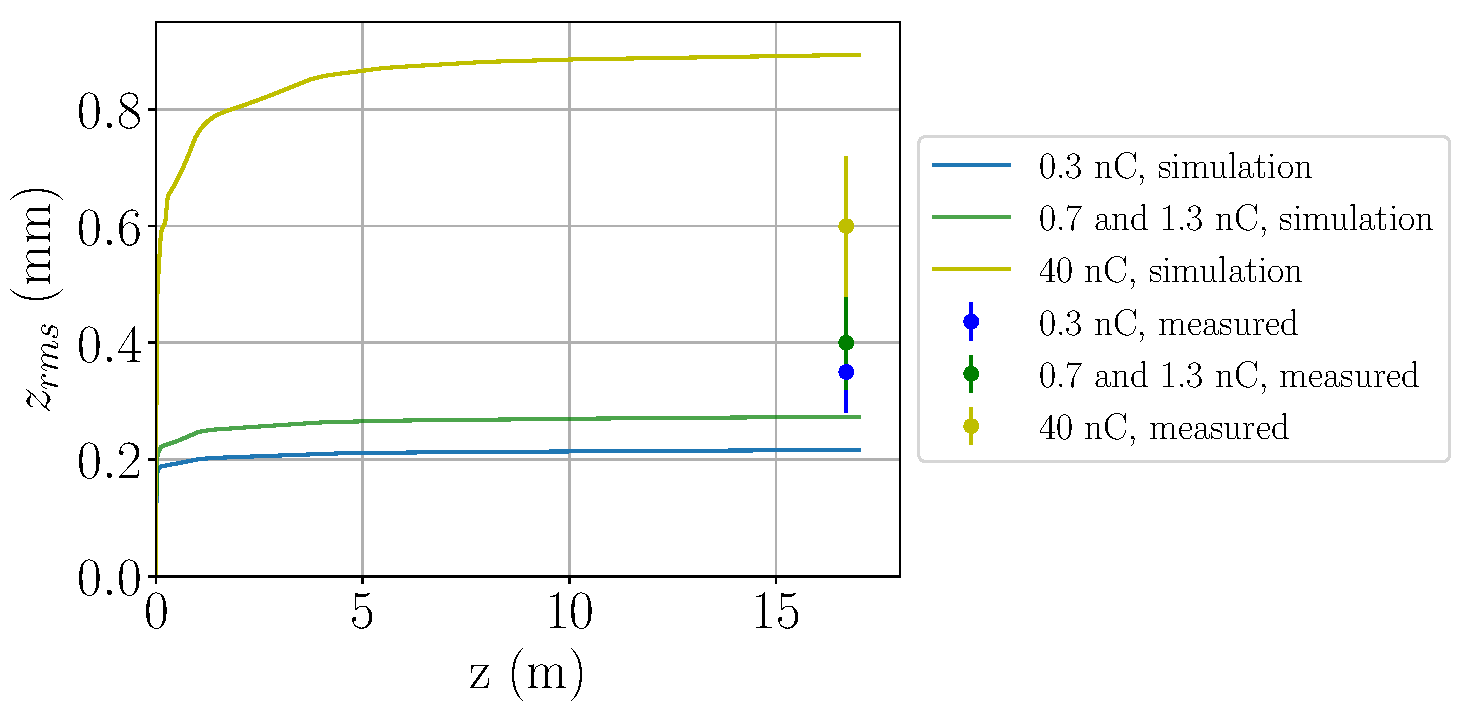
\includegraphics[width=0.8\linewidth]{images/THPMF048f5}
	\caption{Comparison of simulations and experimental measurements.}
	\label{sims}
\end{figure*}
While, we do not have an exact match, the results follow the same trends.
The discrepancies indicate there are still adjustments that can be made
to the simulation model. We will continue to try to improve agreement
as more of these measurements are made. 
This can include better measurements of the beam energy and careful attention to other 
beam line parameters such as the laser radius and solenoid strengths.
In the case of high charge simulations, where the agreement is the worst, 
more consideration is needed for large charge fluctuations in the data.

Experimentally measured values of the bunch duration are shown in Table~\ref{exp}.
Note the units in the table are picoseconds and the units in Fig.~\ref{sims} are millimeters.
The table gives bunch duration, and the plot gives bunch length for the same data.
We hope these can serve as future reference for others doing experiments at the AWA.
\begin{table}[h]
	\centering
	\caption{Experimental Measurements}
	\begin{tabular}{rcc}
		\toprule
		\textbf{Charge} & \textbf{Bunch Dur. (RMS)} & \textbf{Laser spot size}  \\
		\midrule
		\SI{0.3}{nC} & \SI{2.2}{ps} & 4 mm    \\ %[3pt]
		\SI{0.7}{nC} & \SI{2.6}{ps} & 4 mm   \\ %[3pt]
		\SI{1.3}{nC} & \SI{2.6}{ps} & 4 mm    \\
		\SI{30}{nC}  & \SI{4.1}{ps} & 9 mm \\ %[3pt]
		\bottomrule
	\end{tabular}
	\label{exp}
\end{table}




